\documentclass[12pt]{article}

% Variables
\newcommand{\thedate}{March 1, 2012}
\newcommand{\assignment}{CS280 - Spring 2012 HW2}

% Formatting packages
\usepackage{palatino}
\usepackage{fullpage}
\usepackage{fancyhdr}
\usepackage{enumerate}
\usepackage{algorithmic}
\usepackage{pgf}
\usepackage{tikz,tkz-euclide}
\usetkzobj{all}
\usepackage{qtree}
\usetikzlibrary{arrows,automata}

% Math tools
\usepackage{mathtools}
\usepackage{amssymb}
\usepackage{gensymb}
\usepackage{xfrac}

% CS tools
\usepackage{algorithmic}
%\usepackage[options]{mcode}

% Header Settings
\pagestyle{fancy}
\headsep = 15pt
\setlength{\headheight}{60pt}


% Header
\rhead{\textsc{Eric Tzeng, Brandon Wang \\\footnotesize{eric.s.tzeng@gmail.com, brandonwang@berkeley.edu}\\\footnotesize{\thedate} \\}}
\lhead{\Large \textsc{\assignment}}
\cfoot{\large\thepage}

% Numbered environments
\newtheorem{theorem}{Theorem}[section]
\newtheorem{lemma}[theorem]{Lemma}
\newtheorem{proposition}[theorem]{Proposition}
\newtheorem{corollary}[theorem]{Corollary}

% Unnumbered environments
\newenvironment{proof}[1][Proof]{\begin{trivlist}
\item[\hskip \labelsep {\bfseries #1}]}{\end{trivlist}}
\newenvironment{definition}[1][Definition]{\begin{trivlist}
\item[\hskip \labelsep {\bfseries #1}]}{\end{trivlist}}
\newenvironment{example}[1][Example]{\begin{trivlist}
\item[\hskip \labelsep {\bfseries #1}]}{\end{trivlist}}
\newenvironment{remark}[1][Remark]{\begin{trivlist}
\item[\hskip \labelsep {\bfseries #1}]}{\end{trivlist}}

% QED Symbol
\newcommand{\qed}{\nobreak \ifvmode \relax \else
      \ifdim\lastskip<1.5em \hskip-\lastskip
      \hskip1.5em plus0em minus0.5em \fi \nobreak
      \vrule height0.75em width0.5em depth0.25em\fi}

% Start of document
\begin{document}
\section*{Q1: Raw Pixel}
  All graphs in this homework plot the number of samples as the x-axis, and the 
  error rate as the y-axis.
  \begin{enumerate}[a.]
    \item \quad \\
      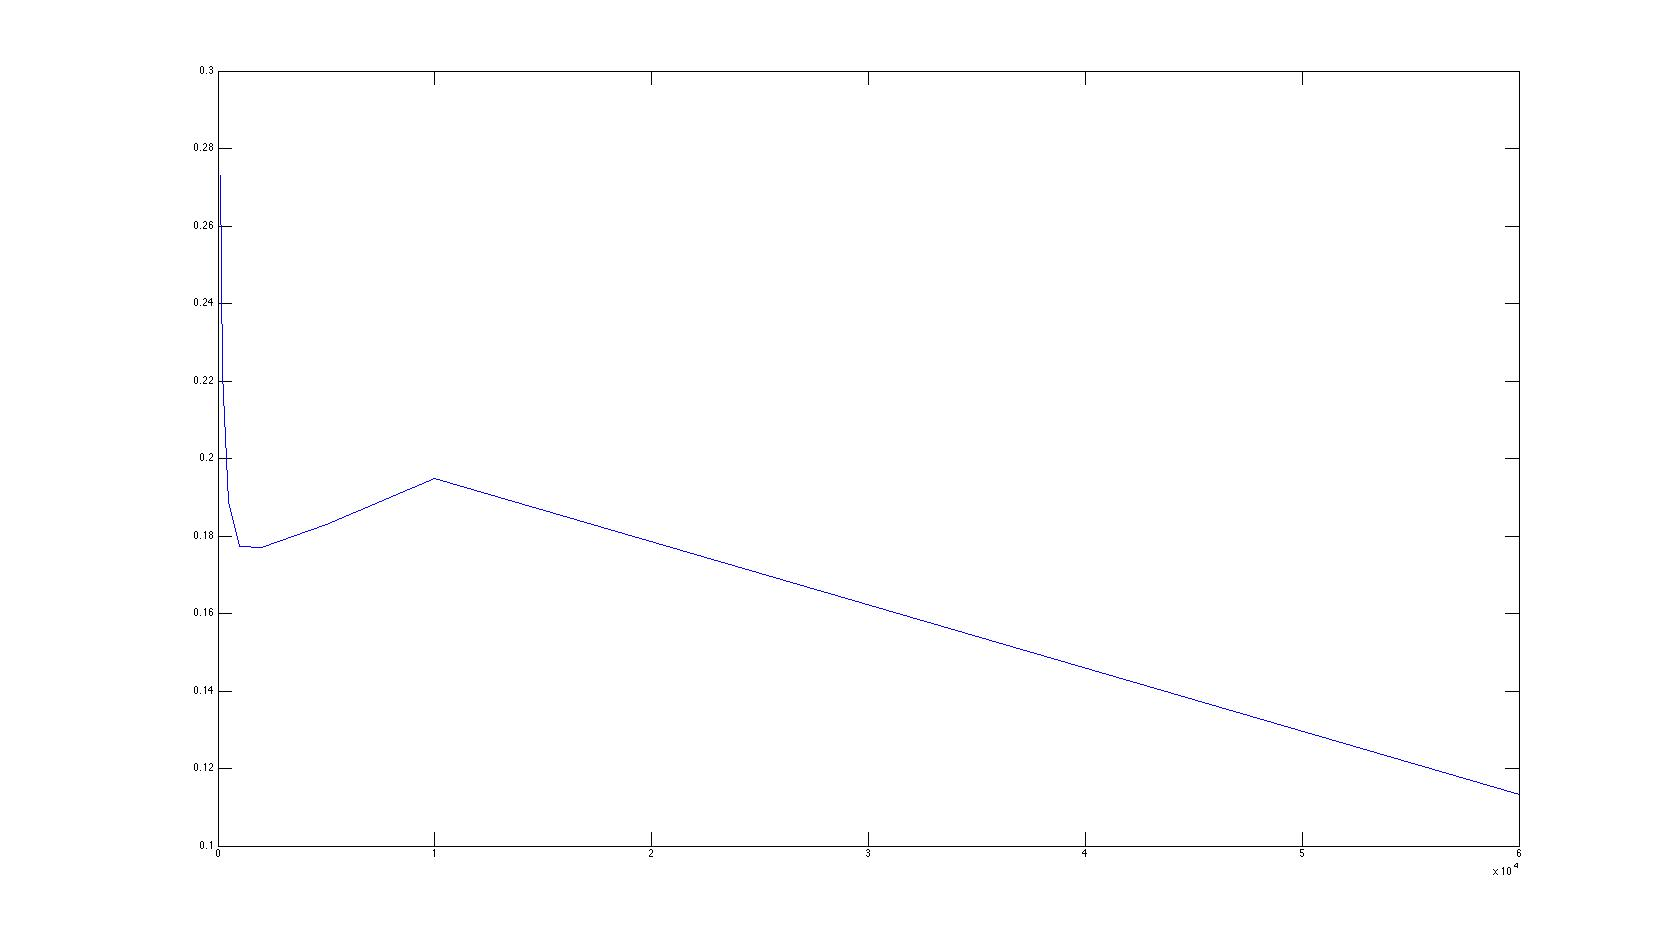
\includegraphics[scale=0.35]{q1_pixel_error.jpg}
      \begin{tabular}{l|l}
        \hline
        Training Samples & Error Rate \\
        \hline
        100   & 0.2731 \\
        200   & 0.2219 \\
        500   & 0.1889 \\
        1000  & 0.1774 \\
        2000  & 0.177  \\
        5000  & 0.1829 \\
        10000 & 0.1949 \\
        60000 & 0.1134 \\
      \end{tabular}
  \end{enumerate}
\newpage
\section*{Q2: Spatial Pyramids}
  \begin{enumerate}[a]
    \item Adding spatial pyramid features should help over raw pixel values for
      a number of reasons. First, using pyramids allows us to examine an image
      at a number of different scales (where larger pyramids correspond to
      smaller scales). Second, using pyramids at various levels also performs
      smoothing on the image. Even if there is an isolated errant pixel, at
      larger window sizes such as $7 \times 7$, this lone pixel's intensity will
      hardly make a difference, since we are summing 49 pixels
      together. Essentially, high intensity pixels that are grouped with other
      high intensity pixels will stay high intensity with larger window sizes,
      whereas lone high intensity pixels will be smoothed out.
    \item \quad \\
      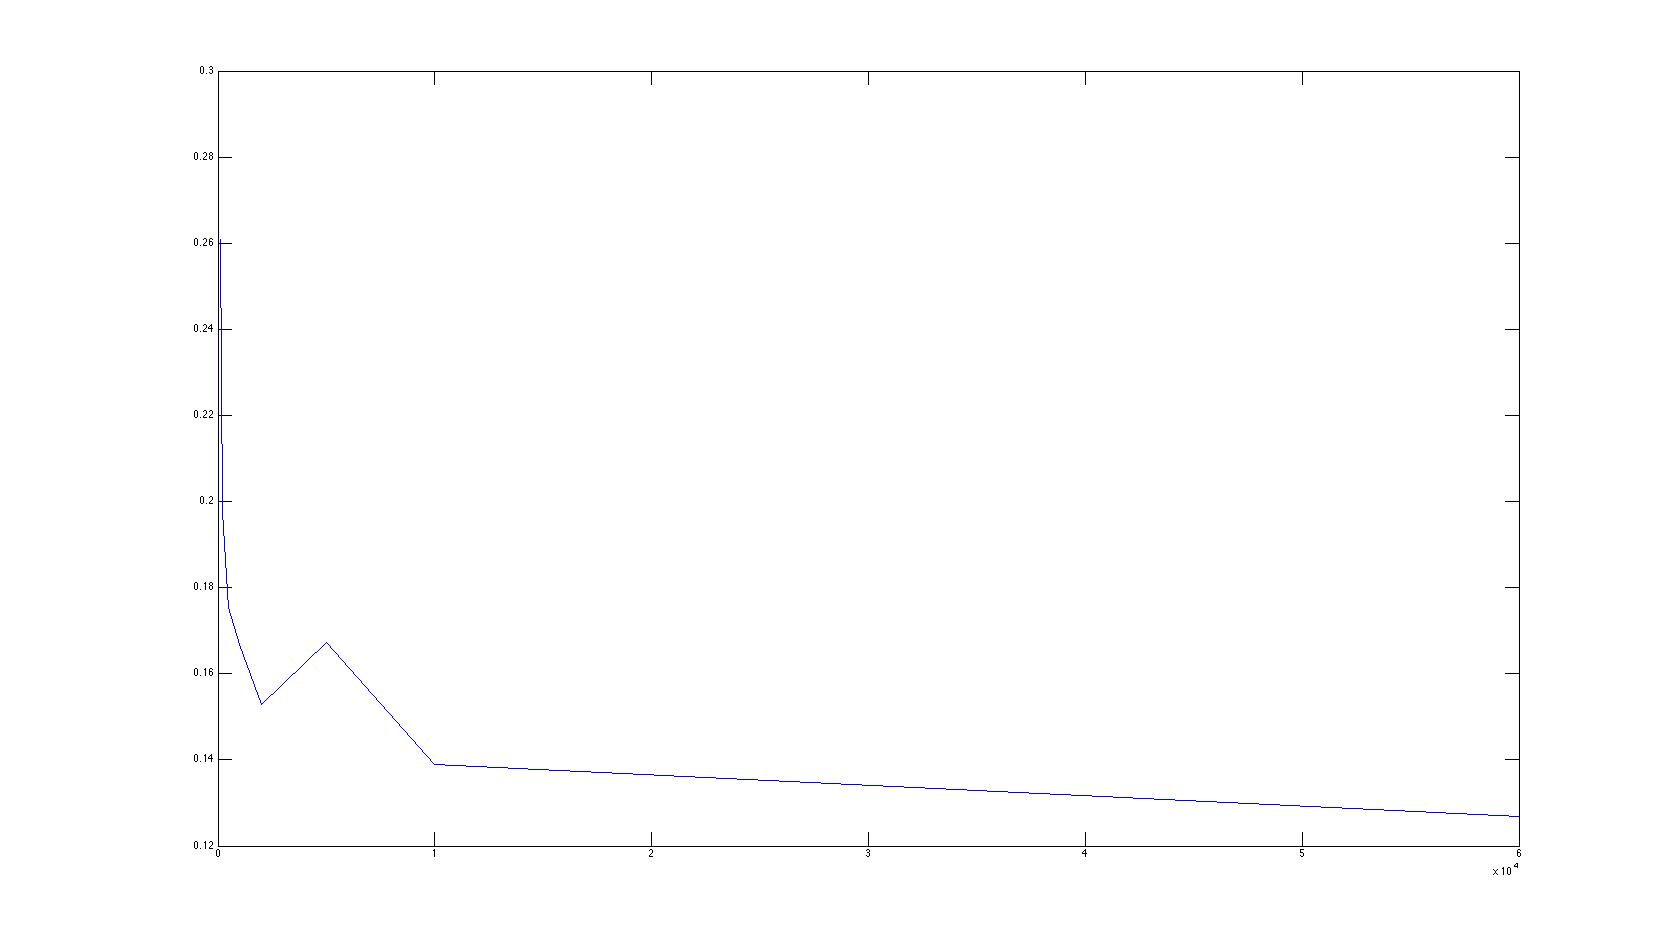
\includegraphics[scale=0.35]{q2_full.jpg}
      \begin{tabular}{l|l}
        \hline
        Training Samples & Error Rate \\
        \hline
        100   & 0.2608 \\
        200   & 0.1975 \\
        500   & 0.1754 \\
        1000  & 0.1667 \\
        2000  & 0.1528 \\
        5000  & 0.1672 \\
        10000 & 0.139 \\
        60000 & 0.1269 \\
      \end{tabular}
  \end{enumerate}

\newpage
\section*{Q3: PHOG Normalized Tap Filter}
  \begin{enumerate}[a.]
    \item Gradient orientations capture the orientations of edges in the
      image. Essentially, when we use gradient orientations, we are identifying
      the edges of the digit (and thus the outline). The idea is that the
      distribution and orientations of edges in an image will be a strong
      indicator of what digit is being represented. For instance, a '1' is
      likely to have strong horizontal gradients along the center of the image,
      whereas a '0' is likely to have strong gradients in all directions further
      away from the center.
    \item \quad \\
      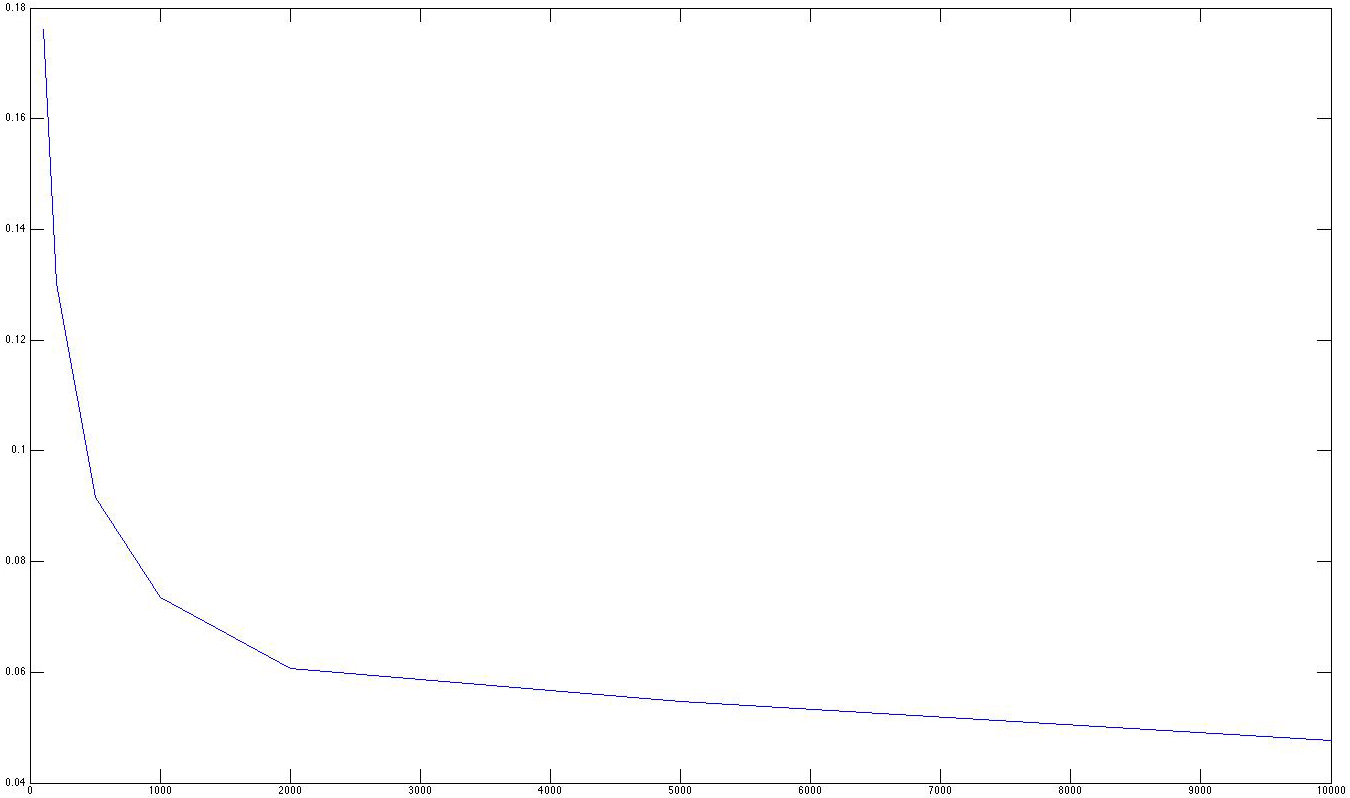
\includegraphics[scale=0.35]{q3_normalized_tap.jpg}
      \begin{tabular}{l|l}
        \hline
        Training Samples & Error Rate \\
        \hline
        100   & 0.1761 \\
        200   & 0.1302 \\
        500   & 0.0916 \\
        1000  & 0.0736 \\
        2000  & 0.0607 \\
        5000  & 0.0548 \\
        10000 & 0.0476 \\
      \end{tabular}
  \end{enumerate}


\newpage
\section*{Q3: PHOG Unnormalized Tap Filter}
  \begin{enumerate}[c.]
    \item Features corresponding to counts in the $7 \times 7$ windows will have
      larger values than features corresponding to counts in the $4 \times 4$
      windows, simply by virtue of the fact that larger windows have more
      pixels. This means that the $7 \times 7$ window features span a larger
      range, which in turn means that distances computed between examples will
      rely more heavily on the $7 \times 7$ features than the smaller $4 \times
      4$ ones. By normalizing, we eliminate this disparity so that each feature
      contributes proportionally to the computed distance. \\
      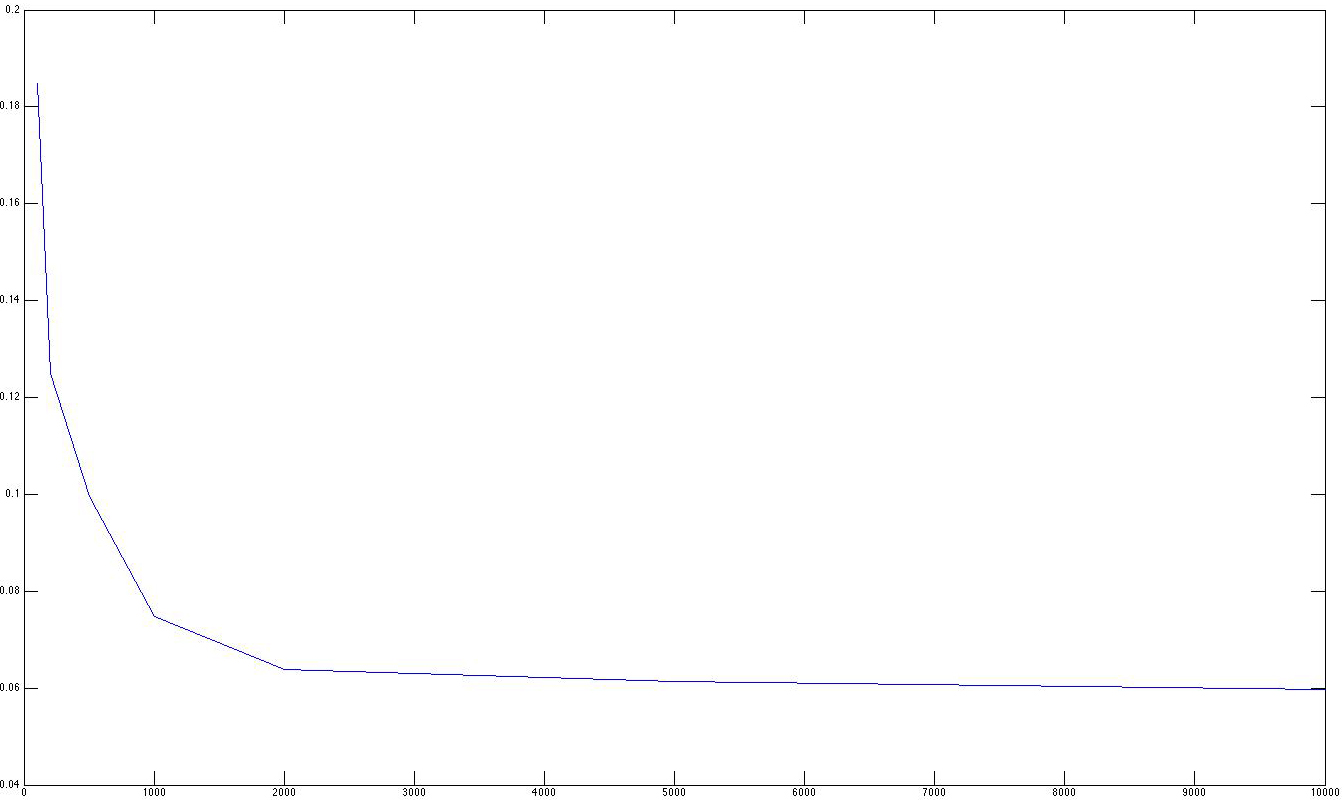
\includegraphics[scale=0.35]{q3_unnormalized.jpg}
      \begin{tabular}{l|l}
        \hline
        Training Samples & Error Rate \\
        \hline
        100   & 0.1849 \\
        200   & 0.1250 \\
        500   & 0.0996 \\
        1000  & 0.0747 \\
        2000  & 0.0638 \\
        5000  & 0.0613 \\
        10000 & 0.0597 \\
      \end{tabular}
  \end{enumerate}

\newpage
\section*{Q3: PHOG Normalized Gauss Filter}
  \begin{enumerate}[d.]
    \item \quad \\
      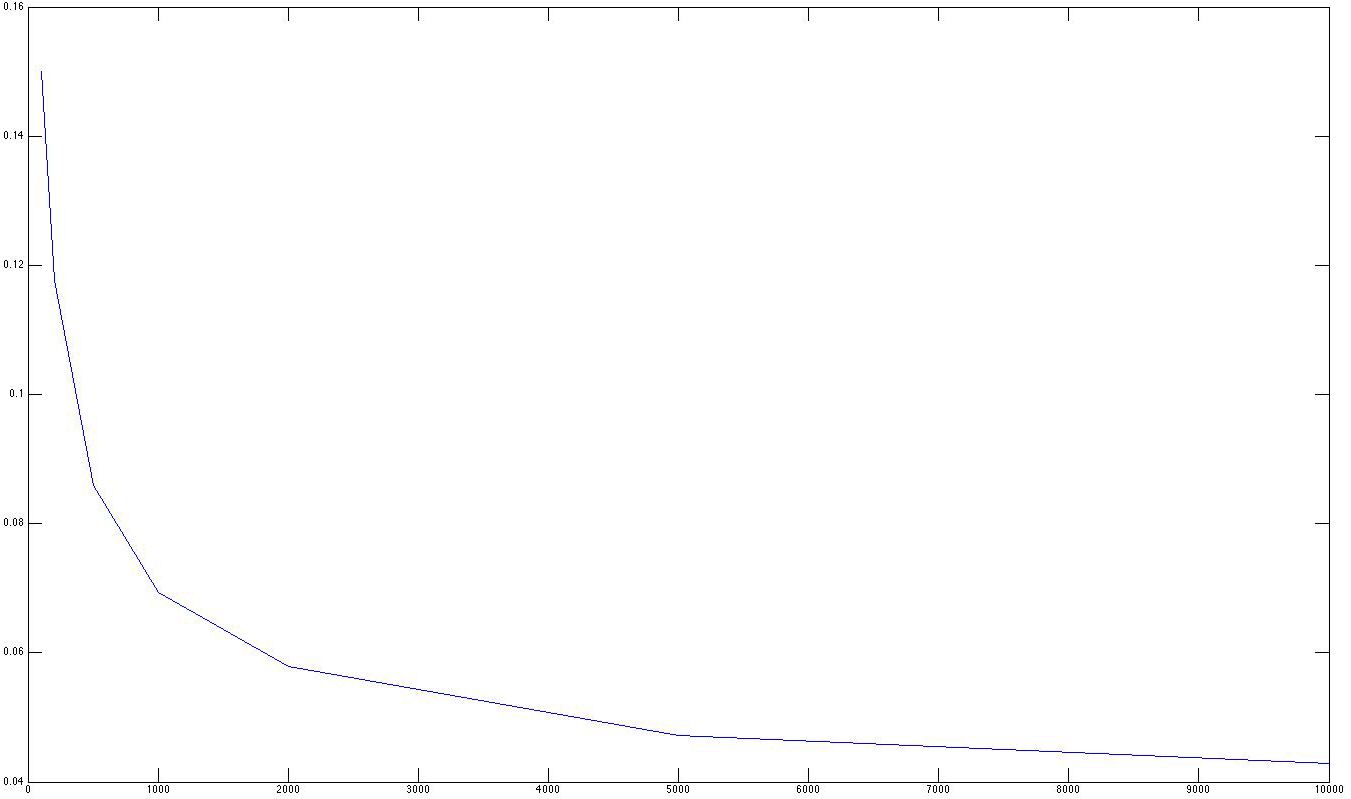
\includegraphics[scale=0.35]{q3_normalized_gauss.jpg}
      \begin{tabular}{l|l}
        \hline
        Training Samples & Error Rate \\
        \hline
        100   & 0.1500 \\
        200   & 0.1176 \\
        500   & 0.0859 \\
        1000  & 0.0693 \\
        2000  & 0.0579 \\
        5000  & 0.0472 \\
        10000 & 0.0429 \\
      \end{tabular}
  \end{enumerate}

\newpage
\section*{Q3: PHOG Normalized Gauss Filter}
  \begin{center}
  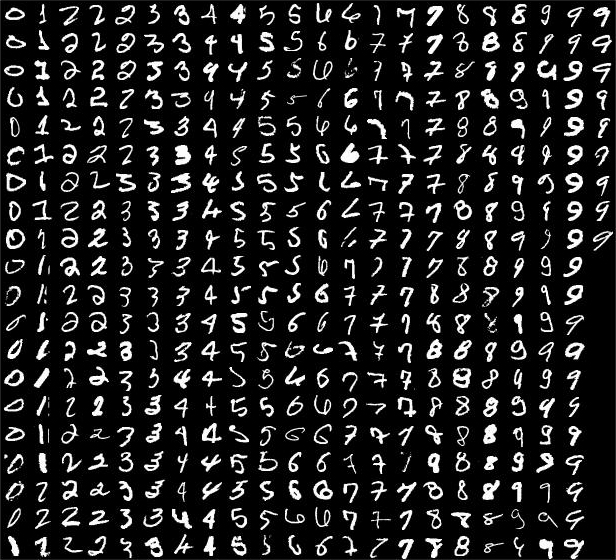
\includegraphics[scale=0.75]{q4_phog_normalized_err.jpg}
  \end{center}
  We believe these errors to be reasonable. 
  As humans, we have issues discerning up to 25\% of these errors, especially
  when there are uncompleted marks, or marks outside of the digit.

\newpage
\section*{Summary}
  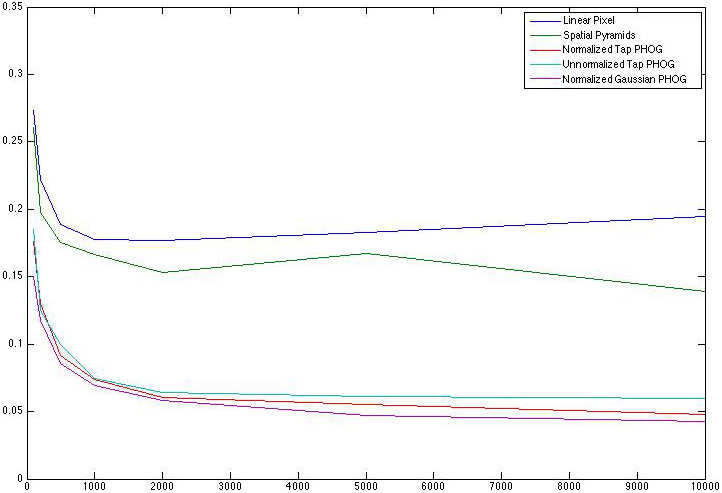
\includegraphics[scale=0.7]{allgraphs_sm.jpg}
  Our Gaussian PHOG filter performed the best, with an error rate of about 4.3\%
   using the 10000-sample training set.

  We used summed area tables in implementing the filters in Matlab. Our program
  trains against the 10000-sample training set in about 3 minutes, and test 
  against the 10000-sample test set in another 3 minutes, allowing us to test 
  our filters using the 7th training set in $train_small.mat$ in about 6 minutes.

\end{document}
